\chapter{Flight data}\label{ch:flight}

The TeleMega recorded the IREC flight in Midland. \file{flightData/cdFlight.py}
calculates from these data the atmosphere of that day, the speed, the drag
coefficient in the coast phase and the conditions of the sweep. It plots the result
against the CFD runs and OpenRocket.

\section{Command}

\begin{shell}
python3 flightData/cdFlight.py [--csv AconcaguaIREC_TeleMega.csv] [--mass 24.52]
        [--runs ~/runs] [--ork rocket.ork] [--alphas 0,8] [--out cdFlight.png]
\end{shell}

\begin{tabularx}{\linewidth}{@{}P{0.24\linewidth} P{0.26\linewidth} L@{}}
\toprule
Option & Default & Function \\
\midrule
\ent{--csv} & \file{flightData/AconcaguaIREC_TeleMega.csv} & TeleMega data. \\
\ent{--mass} & \unit{24.52}{kg} & Mass after burnout, from the OpenRocket simulation. \\
\ent{--runs} & \file{~/runs} & Runs to plot. The script uses the last segment of each run. \\
\ent{--ork} & \file{~/Downloads/207 - Aconcagua.ork} & OpenRocket file for its $C_D$ curve. Optional. \\
\ent{--alphas} & \val{0,8} & Angles of the runs to plot. \\
\ent{--tanchor} & \unit{18}{s} & Time of the speed anchor. \\
\ent{--out} & \file{flightData/cdFlight.png} & Plot. \\
\bottomrule
\end{tabularx}

\section{Method}

\Cref{fig:flight-method} shows the method. All values come from the telemetry,
except the mass.

\begin{figure}[htbp]
  \centering
  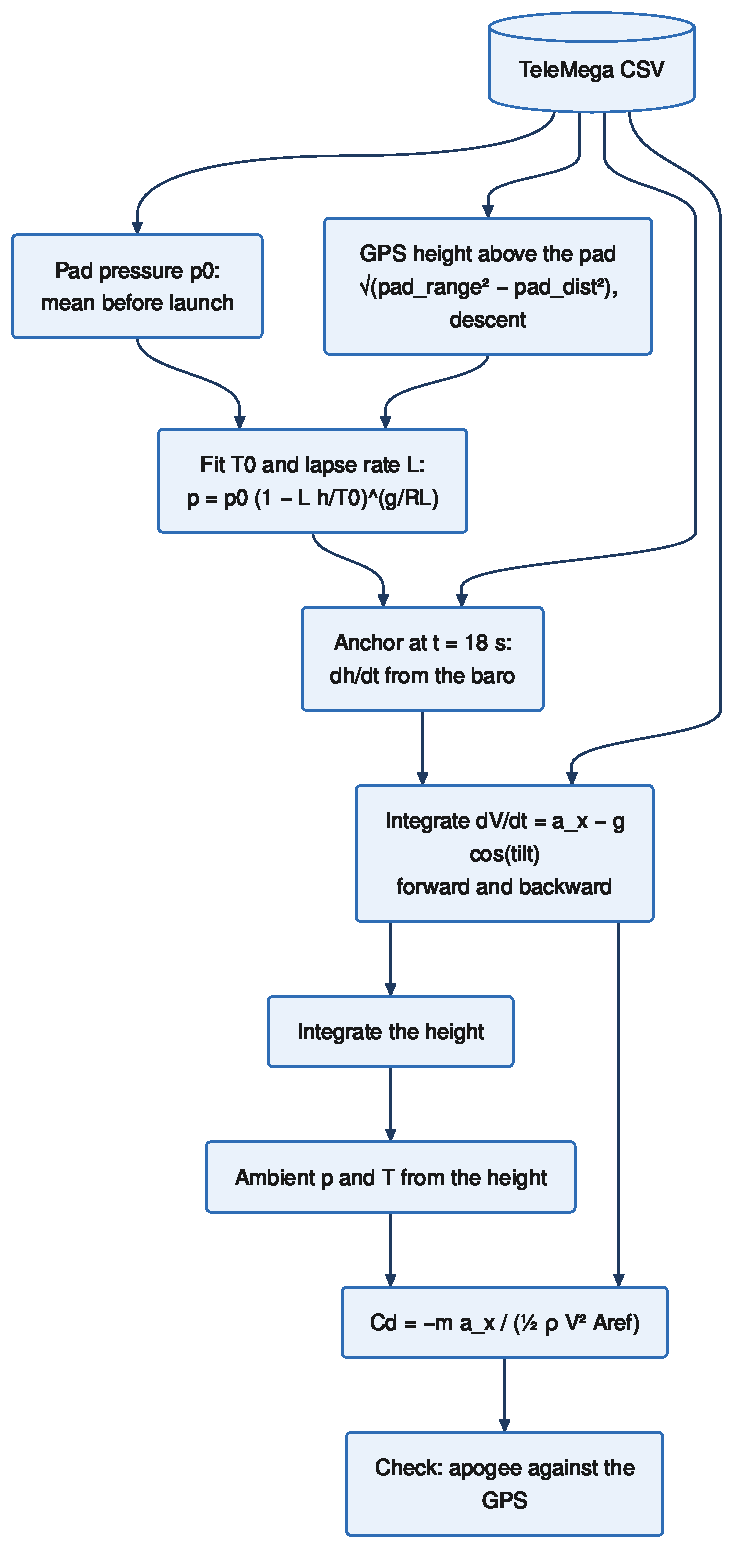
\includegraphics[height=0.5\textheight]{figures/pdf/flight.pdf}
  \caption{Calculation of the flight drag coefficient.}
  \label{fig:flight-method}
\end{figure}

\begin{steps}
\item \textbf{Atmosphere.} The pad pressure $p_0$ is the mean before launch. During
  the descent, the GPS gives the height above the pad,
  $h = \sqrt{\texttt{pad\_range}^2 - \texttt{pad\_dist}^2}$, and the barometer gives
  the pressure without shocks. The script fits $T_0$ and the lapse rate $L$ in
  \[
    p = p_0\left(1 - \frac{L\,h}{T_0}\right)^{g/(R L)}.
  \]
  Result: $p_0 = \unit{90\,565}{Pa}$, $T_0 = \unit{305.0}{K}$,
  $L = \unit{7.2}{K/km}$, from 215 GPS points, with an rms error of 0.3\,\% in
  $\ln p$. The air was approximately \unit{20}{K} warmer than the ISA at all heights.
\item \textbf{Speed.} The script does not use the column \texttt{speed} of the
  TeleMega: its filter converts pressure to height with the ISA, and it gives
  approximately 10\,\% less in the coast. Above $M \approx 0.8$ the barometer is not
  used either, because the static ports are behind shocks. The script integrates the
  axial accelerometer, forward and backward from $t = \unit{18}{s}$:
  \[
    \frac{dV}{dt} = a_x - g\cos\theta_\text{tilt}.
  \]
  At $t = \unit{18}{s}$ ($M \approx 0.65$) the speed comes from the derivative of the
  barometric height with the fitted atmosphere.
\item \textbf{Height and ambient state.} The script integrates $V\cos\theta$ for the
  height, and calculates $p$ and $T$ from the height with the fitted atmosphere.
\item \textbf{Drag.} In the coast, $a_x$ is the axial specific force, so
  $D = -m\,a_x$ and
  \[
    C_D = \frac{-m\,a_x}{\tfrac12\rho V^2 A_\text{ref}}, \qquad
    A_\text{ref} = \pi\,(\unit{0.0755}{m})^2.
  \]
  The script uses the data from $t = \unit{4.0}{s}$, when the residual thrust ends.
\item \textbf{Check.} The integrated apogee is \unit{8137}{m} above the pad. The GPS
  gives \unit{8083}{m} (0.7\,\% difference).
\end{steps}

\section{Results}

\begin{figure}[htbp]
  \centering
  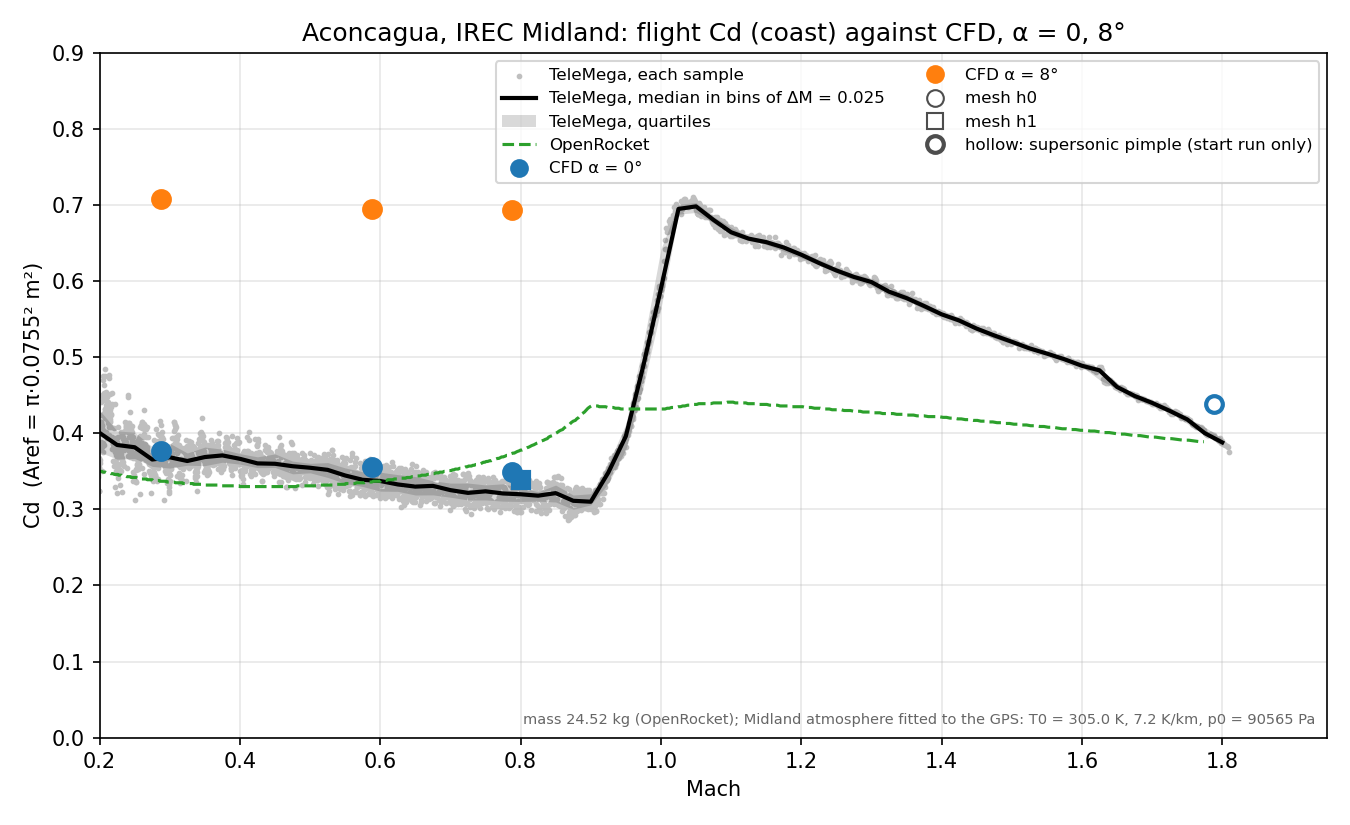
\includegraphics[width=\linewidth]{../../flightData/cdFlight.png}
  \caption{$C_D$ of the flight (coast) against the runs of the first sweep (ISA conditions, \texttt{\textasciitilde/runs.sin-medicion}) and OpenRocket.}
  \label{fig:cdflight}
\end{figure}

\begin{table}[htbp]
\centering
\caption{$C_D$ of the flight and of the CFD at $\alpha = 0$ (first sweep, ISA conditions, 2026-10-17).}\label{tab:cd-flight}
\begin{tabular}{@{}ccccc@{}}
\toprule
$M$ & Flight & CFD & CFD/flight & OpenRocket \\
\midrule
0.3 & 0.369 & 0.376 ($h0$) & 1.02 & 0.336 \\
0.6 & 0.337 & 0.356 ($h0$) & 1.05 & 0.337 \\
0.8 & 0.320 & 0.349 ($h0$), 0.339 ($h1$) & 1.09, 1.06 & 0.378 \\
$\approx$1.03 & $\approx$0.70 (peak) & -- & -- & $\approx$0.44 \\
1.2 & $\approx$0.64 & -- & -- & $\approx$0.43 \\
1.8 & 0.388 & 0.438 (pimple start only) & 1.13 & 0.389 \\
\bottomrule
\end{tabular}
\end{table}

\begin{itemize}
\item From $M = 0.3$ to $0.8$ the CFD is 2 to 9\,\% above the flight, and it decreases
  from $h0$ to $h1$.
\item In the flight, $C_D$ doubles from $M = 0.9$ to $1.0$. OpenRocket does not show
  this peak. No CFD run is in this range yet.
\item The flight value at $M = 1.8$ is 13\,\% below the pimple start run. That run is
  not a result of the central template.
\end{itemize}

\section{Angle of attack in the flight}\label{sec:flight-alpha}

The rocket rolls at approximately 4 revolutions per second in the coast. The mean
lateral acceleration follows the square of the roll rate with a constant radius of
approximately \unit{2.8}{cm}: it is the centripetal acceleration of a sensor off the
axis. An aerodynamic normal force has a fixed direction in space, so in the body axes
it turns with the roll. The oscillation of the lateral acceleration at the roll
frequency gives $C_N \approx 0.01$ to $0.03$. With $C_{N\alpha} \approx \unit{18}{/rad}$
from the CFD, $\alpha < 0.2^\circ$ in all the coast. The sensor noise is in this value,
so it is an upper limit.

\section{Uncertainty}

\begin{tabularx}{\linewidth}{@{}P{0.24\linewidth} L@{}}
\toprule
Source & Effect \\
\midrule
Mass & $C_D$ is proportional to the mass, which is a design value of OpenRocket, not a measurement. \\
Wind & No data. The speed is relative to the ground. \\
Flight path & The gravity term uses the attitude as the direction of the flight path. With $\alpha < 0.2^\circ$ the error is small. \\
Atmosphere & The fit gives one lapse rate from the pad to \unit{8}{km}. The local layers differ from the fit by up to \unit{7}{K}. \\
\bottomrule
\end{tabularx}
